
La idea de random forest utliziar múltiples arboles árboles de decisión para mejorara la eficacia del clasificador.Esto es posible gracias al bajo costos que lleva entrenar y consultar a cada árbol. Este modelo tiene sentido si se utilizan  diferentes árboles que se complementen logrando mayor eficacia.  Para lograr eso los atributos utilizados en las divisiones de los nodo al construir el árbol se limitan a un subconjunto aleatorio de los atributos. El tamaño de ese subconjunto suele determinar la diversidad lograda dentro del bosque. Utilizando mismos parámetros que para el clasificador de un único árbol volvimos a hacer pruebas variando la cantidad de árboles del bosque y el tamaño del subconjunto de atributos a considerar. En la figura ~\ref{fig:forest_f05_en_funcion_de_cantidad_de_arboles} se puede ver claramente que utilizando la raíz cuadrada de la cantidad máxima de atributos como tamaño del subconjunto se obtienen los mejores resultados. Alcanzando la mayo eficacia para bosques de 35 árboles. 


\begin{figure}[H]
    \centering
        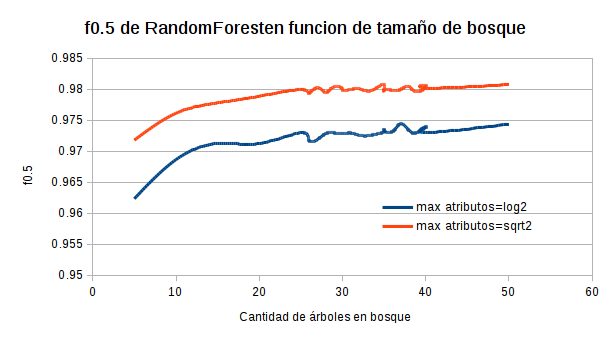
\includegraphics[width=\textwidth]{plots/forest_f05_en_funcion_de_cantidad_de_arboles.png}
        \caption{f0.5 en funcíon de cantidad de árboles}
        \label{fig:forest_f05_en_funcion_de_cantidad_de_arboles}
\end{figure}

